%%%%%%%%%%%%%%%%%%%%%%%%%%%%%%%%%%%%%%%%%%%%%%%%%%%%%%%%%%%%%%%%%%%%%%
%
%Parallel Computing work
%Authors: Michael Reitgruber and Wiedemann Sebastian
%
%%%%%%%%%%%%%%%%%%%%%%%%%%%%%%%%%%%%%%%%%%%%%%%%%%%%%%%%%%%%%%%%%%%%%%

\documentclass[12pt,a4paper,titlepage,oneside]{scrartcl}
\newcommand{\lang}{de}
\usepackage{esseProtocol}
\usepackage{tablefootnote}
\usepackage[parfill]{parskip} % keine blöden Einrückungen bei neuen Absätzen
\usepackage{graphicx}
\usepackage{mathtools}
\usepackage{hyperref}

\lstset{literate=%
{Ö}{{\"O}}1
{Ä}{{\"A}}1
{Ü}{{\"U}}1
{ß}{{\ss}}1
{ü}{{\"u}}1
{ä}{{\"a}}1
{ö}{{\"o}}1
{~}{{\textasciitilde}}1
}

%%%%%%%%%%%%%%%%%%%%%%%%%%%%%%%%%%%%%%%%%%%%%%%%%%%%%%%%%%%%%%%%%%%%%%
%
% FOR STUDENTS
%
%%%%%%%%%%%%%%%%%%%%%%%%%%%%%%%%%%%%%%%%%%%%%%%%%%%%%%%%%%%%%%%%%%%%%%

% Team number or "0" for Lab0
%\newcommand{\team}{19}
% Date
\newcommand{\datum}{20.01.2015}
% valid values: "Lab0", "Lab1" (be sure to use Uppercase for first character)
%\newcommand{\lab}{Lab1}

\newcommand{\lvaname}{Parallel Computing}
\newcommand{\paperitle}{Fast Fourier Transformation}
\newcommand{\lvanr}{184.710}
\newcommand{\semester}{WS 2015}

% Student data in Lab0 or 1. student of team in Lab1
\newcommand{\studentAName}{Michael Reitgruber}
\renewcommand{\studentAMatrnr}{1426100}

% 2. student of team in Lab1, for Lab0 or if your team has less students, remove these 2 lines
\newcommand{\studentBName}{Sebastian Michael Wiedemann}
\renewcommand{\studentBMatrnr}{1425647}


% 5. student of team in Lab1, for Lab0 or if your team has less students, remove these 2 lines
%\newcommand{\studentEName}{Otto Mustermann}
%\renewcommand{\studentEMatrnr}{0236214}

%%%%%%%%%%%%%%%%%%%%%%%%%%%%%%%%%%%%%%%%%%%%%%%%%%%%%%%%%%%%%%%%%%%%%%
%
% DO NOT CHANGE THE FOLLOWING PART
%
%%%%%%%%%%%%%%%%%%%%%%%%%%%%%%%%%%%%%%%%%%%%%%%%%%%%%%%%%%%%%%%%%%%%%%

\newcommand{\colormode}{color}
%\newcommand{\dokumenttyp}{Abgabedokument \lab}

\begin{document}

\maketitle
\setcounter{section}{0}
\setcounter{tocdepth}{2}
\tableofcontents
\pagebreak
%%%%%%%%%%%%%%%%%%%%%%%%%%%%%%%%%%%%%%%%%%%%%%%%%%%%%%%%%%%%%%%%%%%%%%
%
% CONTENT OF DOCUMENT STARTS HERE
% DON'T MODIFY, IF NOT NECESSARY ! EVERYTHING IS IN ITS OWN MODULE!
%
%%%%%%%%%%%%%%%%%%%%%%%%%%%%%%%%%%%%%%%%%%%%%%%%%%%%%%%%%%%%%%%%%%%%%%
%EXAMPLE
\section{Introduction}
	\subsection{Correctness}
	FFT = FFT/2 +FFT/2
	\subsection{Complexitiy}
	\subsubsection{iterative method}
\begin{lstlisting}
<inplace splitting> - O(n)
for(int i = 2; i <= len; i *= 2) - O(log(n))
	for(int k = 0; k < i/2; k++) - O(i/2)
		for(int j = 0; j < len/i; j++) - O(n/i)

\end{lstlisting}
Simple to analyse:
\begin{math}
O(n + log(n) * i/2 * n/i) = O(log(n)*n)
\end{math}
\subsubsection{recursive method}
\begin{lstlisting}
   if(step >= len)
      return;
    fft_help(dc2, dc1, len, step*2); - O(log(n-1))
    fft_help(dc2+step, dc1+step, len, step*2); - O(log(n-1))
    for(int k=0; k<len/2; k+=step) -- O(n)
\end{lstlisting}
\begin{math}
O(2*log(n-1) * n) = O(log(n)*n)
\end{math}\newline
This is visualized with memory pattern in 1.2
	\pagebreak
	\subsection{Memory Access Pattern}
	Basicly, the recursive implementation calculates the odd and even part of the FFT like a binary tree. All left nodes in the recursive call tree calculate the even part and the odd part is calculated by the right nodes. Parent nodes need the children's result for their own calculations. That's why our arrays get swapped. 
The resulting memory access pattern is as follows:
\begin{center}
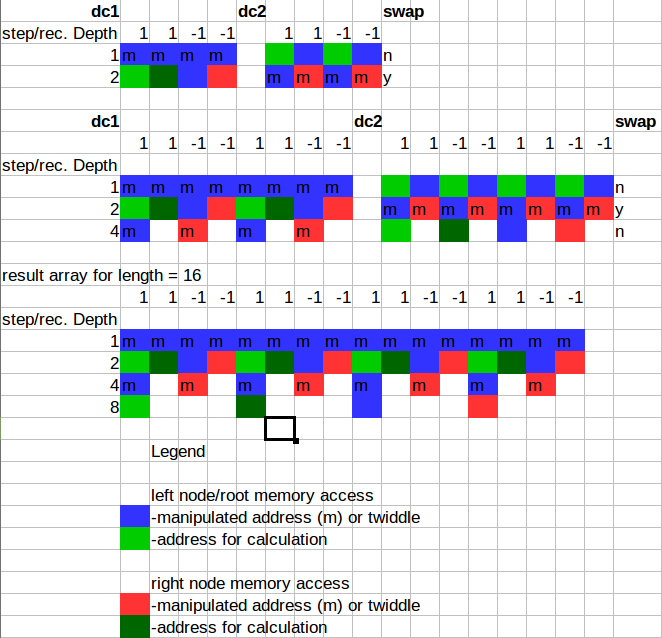
\includegraphics[width=\textwidth]{memacc.png}
\end{center}
The 1's and -1's are just from an example rectangle signal. The picture shows the full memory access for arrays of length 4 and 8. This information is all that you need since you can easily iterative expand the access picture in two steps:
\begin{enumerate}
\item duplicate the memory pattern horizontally
\item copy the last line of the other array, add double the "whitespaces" + 1 after the single accesses and add it as last line of the new access pattern. 
\end{enumerate}
As example we also included the result array for length = 16.

\section{Fourier Transformation}
	Our implementations need input of the length of \(2^{n}\).
	\subsection{discrete Implementation}
	We use the simple DFT algorithm. It calculates the sum of all input variables multiplied with their roots of unity and does that for each output index.
	\subsection{iterative FFT Implementation}
	We implemented an inplace bottom-up FFT. We fill the array in bit reversed order. This splits the array in odd and even parts, before the algorithm starts the actual FFT. That is called \textit{In-place splitting}. The in-place splitted array also represents the FFT of all single elements, which is the element itself. The three loops then are combining the transforms in place. 


	\subsection{recursvie FFT Implementation}
	Basicly our implementation calculates FFT for the odd and even part and stores the result in one array, recursive calls later use these previous calculations, to calculate further. That is why the two arrays get swapped. It is easily to demonstrate if you draw youself the tree of recursive calls. Each node with two children gets their needed FFT information, calculated by the children, stored in array 1. Each node self stores the calculated information in array 2, which
is array 1 in all parents and the output array in the original call. 
	\subsection{Sequential Performance}	
	The experimental estimation for which our FFT becomes faster than the trivial DFT algorithm:
\begin{center}
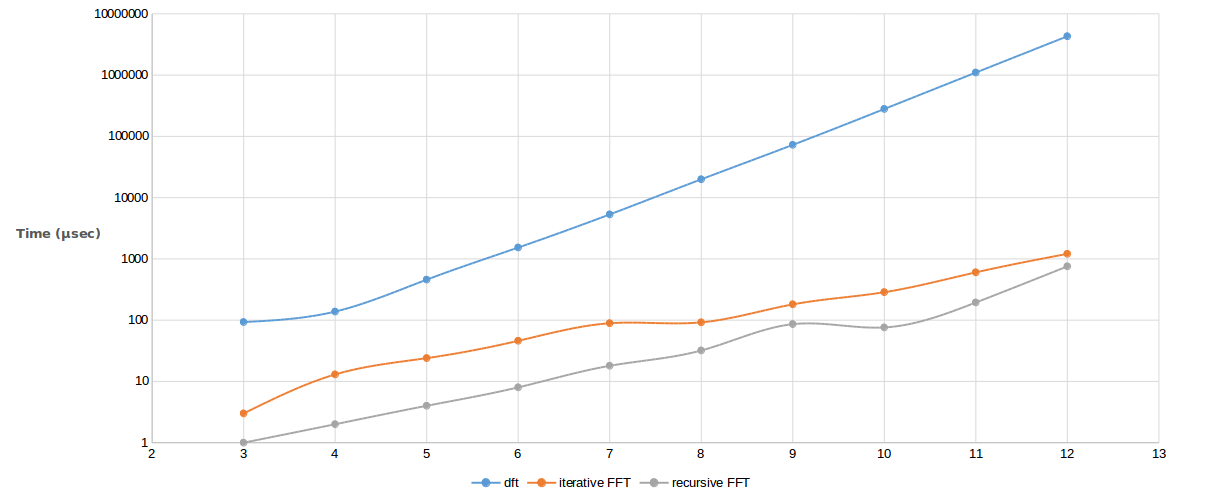
\includegraphics[width=\textwidth]{dft_comp.png}
\end{center}
Our FFT is faster from the beginning on.

Here is a comparison of Jupiter's and Saturn's performance of our iterative FFT. We did not include the recursive versions, since it is ways slower after \(2^{14}\) numbers.
\begin{center}
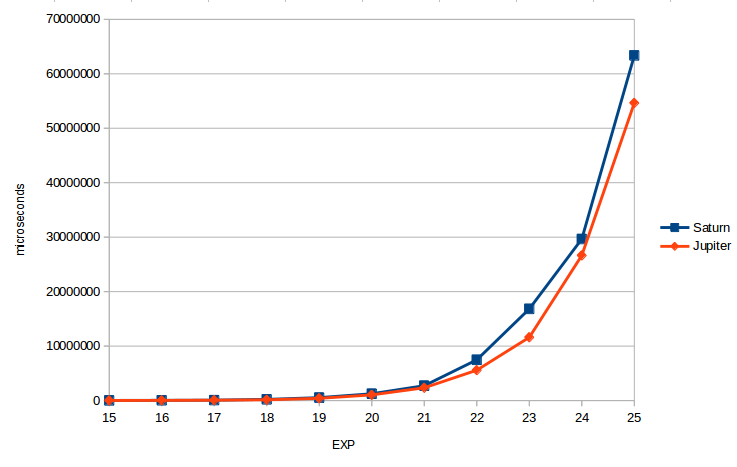
\includegraphics[width=\textwidth]{seq_performance.png}
\end{center}
As expected, Jupiter is faster because it has CPUs. We used this information for our speedup plots later at our parallelism problem solutions.
\section{OpenMP}
	\subsection{Recursive Implementation}
	\subsubsection{Implementation}

Only a small change to the calling code of the fft, as well as the way the recursive calls are made is needed to adapt the recursive implementation to use OpenMP.

\textbf{Calling Code:}
\begin{lstlisting}
  #pragma omp parallel shared(timeUsed, in, out, len)
  {
    #pragma omp single
    {
      fft(in, out, len);
    }
  }
\end{lstlisting}

\textbf{Recursive Calls:}
\begin{lstlisting}
  #pragma omp task final(((len/2)/step) < 1024)
  {fft_help(dc2, dc1, len, step*2);}
  #pragma omp task final(((len/2)/step) < 1024)
  {fft_help(dc2+step, dc1+step, len, step*2);}
  #pragma omp taskwait
\end{lstlisting}

\textbf{Description of \#pragma statements}
\begin{lstlisting}
#pragma omp parallel shared(timeUsed, in, out, len)
\end{lstlisting}
Defines a parallel section which will be executed by all existing threads and tells OpenMP that the variables timeUsed, in, out and len should be shared amongst all threads.

\begin{lstlisting}
#pragma omp single
\end{lstlisting}
Defines a section which will only be executed by a single thread. This ensures that only one thread executes the recursive calls and creates the tasks. Otherwise the same task will be created by multiple threads.

\begin{lstlisting}
#pragma omp task final(((len/2)/step) < 1024)
\end{lstlisting}
Defines a task, which will be put into a taskpool where it is available for execution by another thread. If the condition in the final clause evaluates to true,
this task, and all further tasks created by it, will be executed immediately by the encountering thread. This reduces the overhead of putting the task into the pool.

\pagebreak
\begin{lstlisting}
#pragma omp taskwait
\end{lstlisting}
Tells OpenMP to wait here until the two tasks created above are completed. This is needed to ensure the correct order of execution for the Fast Fourier Transform.

\subsubsection{Performance}
The following graphs show the speedup relative to our fastest sequential implementation.

Average speedup:

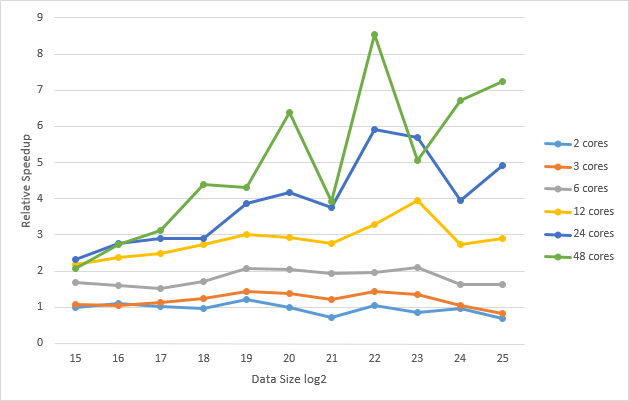
\includegraphics[width=\textwidth]{omp_rec_avg.png}

\pagebreak
Best observered speedup:

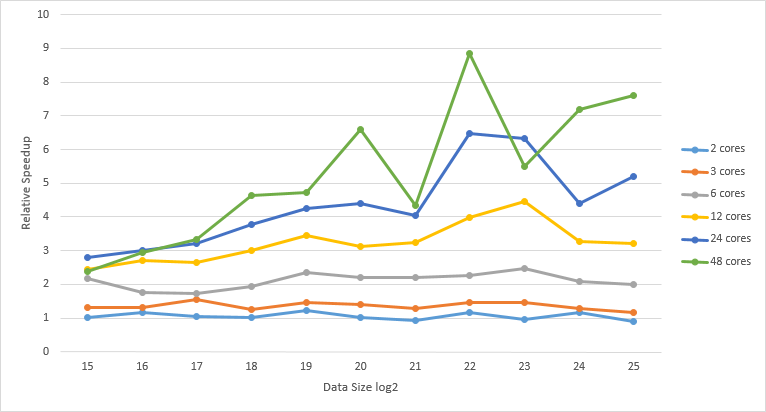
\includegraphics[width=\textwidth]{omp_rec_best.png}

What we can see here is that the speedup for larger amount of cores depends especially on the amount of data supplied.
The greater the amount of data supplied to the algorithm, the greater the amount of tasks created by the program. Further down the recursion tree this leads to the creation of
a large number of tasks, for which there is very little to compute. This would lead to a slowdown because of the overhead associated with switching threads and assigning tasks to threads.
We tried to mitigate this effect by introducing the cutoff value. 1024 was chosen as the value, that delivered the best results during testing. Larger cutoff values led to higher amounts of computation to be done and thus lower speedups overall.
But even with this cutoff there is a drop in speedup after \(2^{23}\) which seems to be the point at which the thread scheduling overhead takes over again.

	\subsection{Iterative Implementation}
	\subsubsection{Implementation}

To adapt the iterative implementation to use OpenMP, we only needed to add the following pragma to the middle for loop in the main FFT body:

\begin{lstlisting}
  #pragma omp parallel for schedule(guided)
  for(int k = 0; k < i/2; k++) {
\end{lstlisting}

This pragma defines a parallel section and tells OpenMP to split the iterations of the following for loop up for all encountering threads. The schedule clause determines in which way the loop will be split.
We tried 3 different schedule options (static, dynamic, guided) from which guided was the one that led to the best performance (closely followed by static scheduling). With this clause the first encountering thread
gets a chunk of the whole iteration space proportional to the amount of threads, each following thread gets a chunk of the remaining iteration space, again proportional to the number of threads. The schedule clause can also take
another paramter called the chunk size, which specifies the minimum size for the chunks. The default value for guided scheduling is approximately loopcount/number\_of\_threads, which is what we use in our implementation.

\subsubsection{Performance}

We did 100 repetitions and took the median as 'average' speedup, since some testcases sometimes completely destroyed the result. Further more the median wasn't always that far apart from the minimum.\newline 
Average speedup:

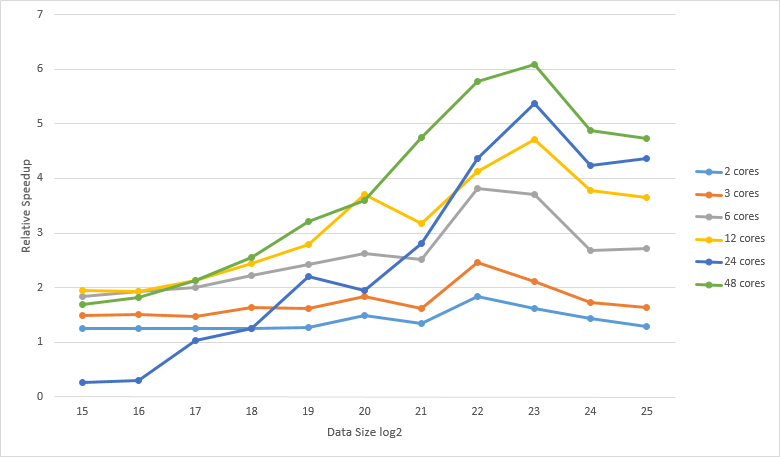
\includegraphics[width=\textwidth]{omp_it_avg.png}

\pagebreak
Best observered speedup:

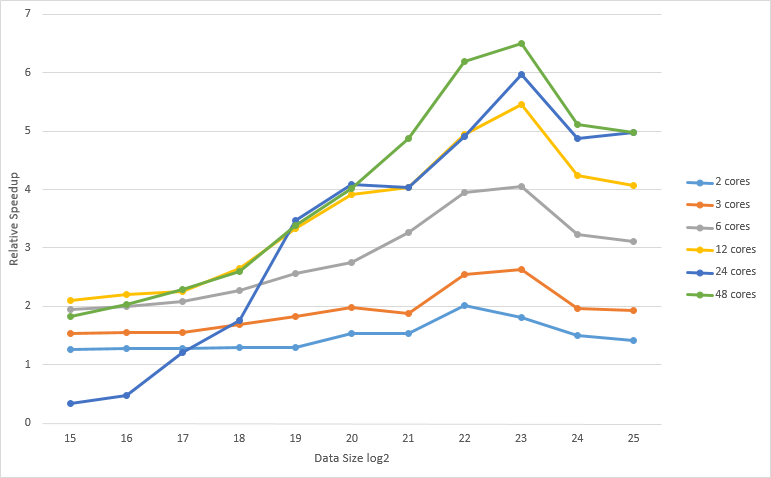
\includegraphics[width=\textwidth]{omp_it_best.png}

As expected we see the same kind of speedup curve as for the recursive implementation, but with the speedup not quite reaching the same values. Probable causes for this could be possibly higher overhead associated with the scheduling, as well as the different memory access pattern,
but we could not determine the actual cause with certainty.

	
\section{cilk}
	\subsection{Recursive Implementation}
	\subsubsection{Implementation}
To adapt the trivial recursive implementation to use cilk, only two new keywords have to be added to the calling code of the recursions:

\textbf{Recursive calls:}
\begin{lstlisting}
  cilk_spawn fft_help(dc2, dc1, len, step*2);
  cilk_spawn fft_help(dc2+step, dc1+step, len, step*2);
  cilk_sync;
\end{lstlisting}

cilk\_spawn tells cilk that the function call (here the recursive calls to fft\_help) can be executed in parallel to the calling function. It is important to note that while the cilk\_spawn keyword permits parallelism, it does not explicitly create a thread. It tells the runtime that the part after the keyword can be executed by another worker. 

cilk\_sync  tells the runtime that all child functions spawned until this point must be completed before the execution can continue past this point. In our case this means that both recursive calls must be completed before the program can continue. 

\textbf{Cutoff}
In addition to the trivial parallelism we also implemented a cutoff threshold after which the remaining parts of the fft will be executed sequentially. 

This can be seen here (with sequential being the same recursive funtion, without the cilk\_ statements: 
\begin{lstlisting}
if((len/2)/step < 64) { //cutoff
		sequential(dc1, dc2, len, step);
		return;
	}
\end{lstlisting}

\subsubsection{Performance}

Average speedup:

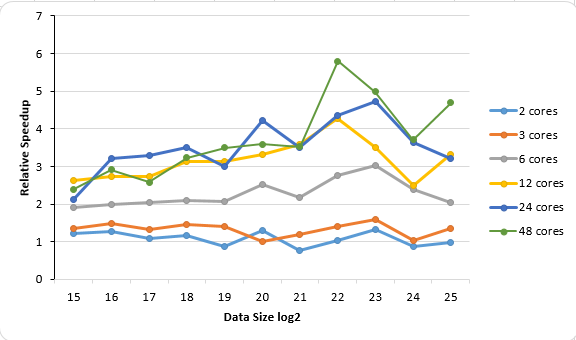
\includegraphics[width=\textwidth]{cilk_rec_avg.png}

Best observered speedup:

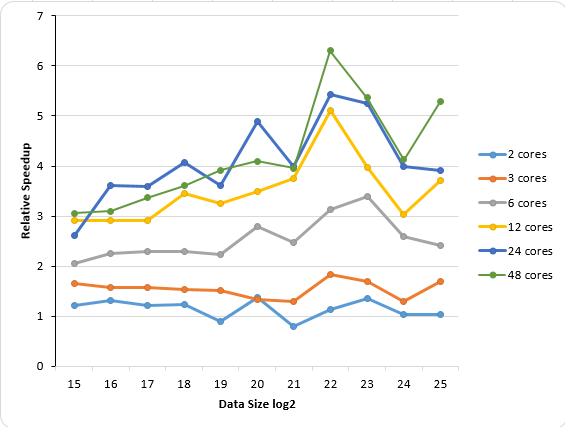
\includegraphics[width=\textwidth]{cilk_rec_best.png}

The graphs again show the same pattern for the speedup, that was already present for both OpenMP implementations, but with a few noticable differences.

First of all the corellation between data size and speedup for larger amounts of cores seems to be lower. We assume this is due to the cutoff having less of an ill effect in the cilk runtime, since even before we get to this point there may already have been parts of the fft executed sequentially, due to the way the cilk\_spawn keyword works. 

Furthermore there is less of a noticable difference speedup between the higher amounts of cores (especially between 24 and 48 cores). We did not find a plausible reason for this in our implementation, but we suspect it might be due to the cilk runtime on the testing server running into problems with higher ammount of cores. This suspicion is supported by the fact that running the cilk program on the server led to high amount of system cpu time used on all cores, while only one core was doing work, which can be seen in the following screenshot: 

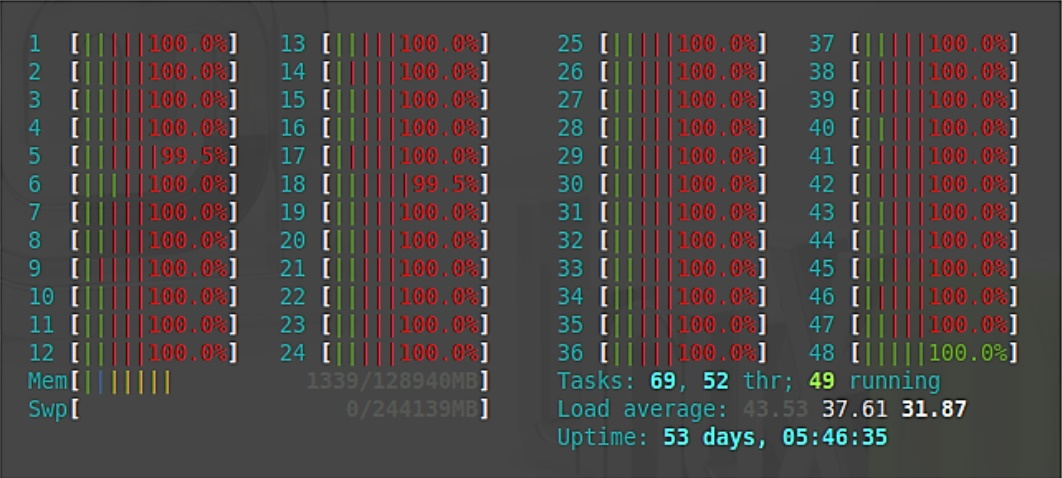
\includegraphics[width=\textwidth]{cpu_util_cilk.jpg}


\section{MPI}
	\subsection{Implementation}
	\subsection{Main implementation}
After many tries and research we came up with a really simple method of dealing with the MPI problem. Our method needs in addition to the number of elements also a processor amount of a power of two. We used the iterative FFT method as base. Since the FFT splits the array into even and odd parts, we used this to our advantage. There are actually just two notable parts of the algorithm which are doing the "MPI-things":
\begin{lstlisting}
for(int k=rank;k < i/2;k+=size)
\end{lstlisting}
This is the second of the three \textit{for} loops in the iterative algorithm. This splits the loop into evenly sized work-parts. Each iteration never crosstalks, which is perfect for parallelism.\newline
The second important part:
\begin{lstlisting}
if(i <= size && rank < i)
	sprayData(i, len);
\end{lstlisting}
\begin{lstlisting}
if(rank +i/2 < i){
	MPI_Send(out, len, MPI_DOUBLE_COMPLEX,
			rank + i/2, rank,MPI_COMM_WORLD);
}else{
	MPI_Recv(out, len, MPI_DOUBLE_COMPLEX,
			 rank - i/2, rank-i/2, MPI_COMM_WORLD, &status);
}
\end{lstlisting}
This basicly sends information to the processor, which is supposed to calculated the odd part of rank's array. 
\subsection{additional implementation}

The algorithm we use lets some processors just wait till the lower rank processors are done. So we tried to avoid that and let all processors, which aren't working on the second ('k'-)loop, help each other in the inner ('j'-)loop. In theory this would let to the result of linear speedup, but sadly MPI\_Scatter and MPI\_Gather are super slow. We also only benchmarked method \textit{help2}. \textit{help} only uses MPI\_Send/Recv but does the equivalent. In early testing we just proved that 'advanced' MPI functions deliver better performance, as told in the lecture.

\subsection{Performance}

Since we need a cores amount of a power of two, we chose 32 jupiter hosts and evenly spread the cores. We didn't bother comparing e.g. 8 cores on one node and 1 core per 8 nodes, because we noticed some strong time differences in the early testphase. \newline
Here is a graph trying to show the relation between the time MPI\_Send and MPI\_Recv needs in relation to len/2 random iterations (max iterations of inner loop):
\begin{center}
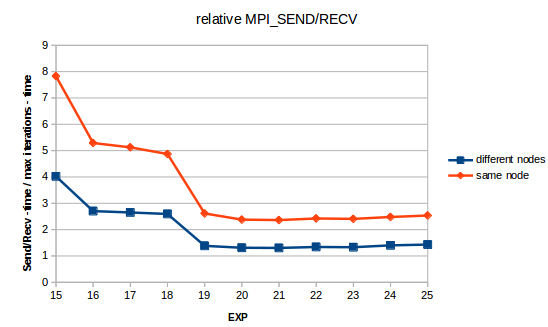
\includegraphics[width=\textwidth]{MPI_sr}
\end{center}
Communication between cores on the same node is obviously far slower. We do not know why there's this slope at 18-19. It always occurs and even on our speedup graphs you can see a hike around this area. 
\newline
Average speedup:
\begin{center}
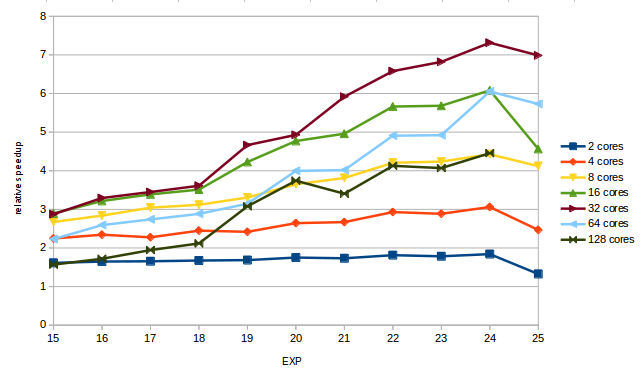
\includegraphics[width=\textwidth]{MPI_med}
\end{center}
Our best observed speedup:
\begin{center}
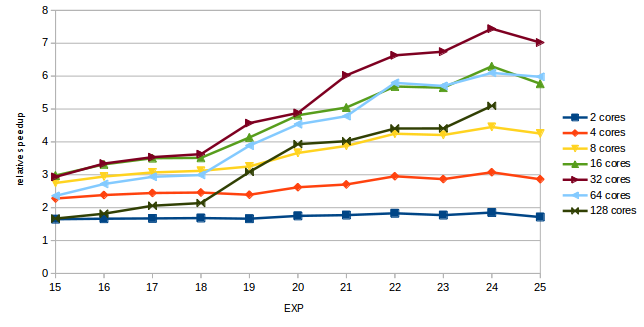
\includegraphics[width=\textwidth]{MPI_best}
\end{center}

Generally our MPI method loses a lot of time during the send and receive phase, especially at low exponents, where all iterations together are faster than the splits. As we kind of expected, most curves are rising in speedup. Similar to openMP and cilk but much smoother. This is most likely because of our simple split method which just works at the beginning and then lets all the cores do the rest without hard disturbance (fewer cores/node \(\implies\) fewer cache problems). \newline


We also include the best-case speedup-graph of our \textit{help2} method:
\begin{center}
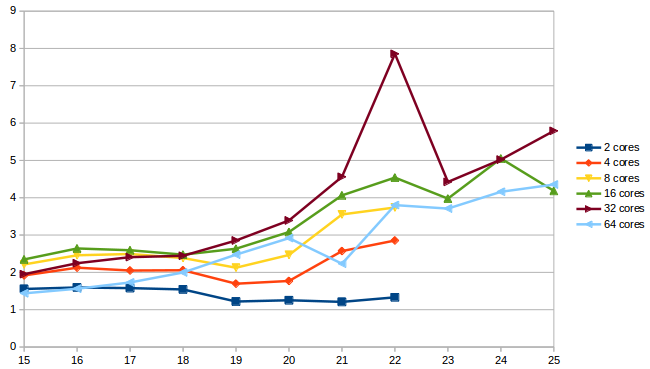
\includegraphics[width=\textwidth]{MPI_help2}
\end{center}

Out of hundred testcases there was one remarkable good one at \(2^{22}\) numbers. Even though MPI\_Scatter/Gather seem to be slow, which can be seen at the beginning of the graph in comparison to the other MPI graphs, it still catches up very nice at larger data amounts.
   
\subsection{Expectation}
We would expect an approximate linear speedup for large enough numbers. We tried to come up with a formula

There are \(2^{p}\) cores and array has length = \(2^{n}\)\newline
A ... average time needed for len/2 (=\(2^{n-1}\)) operations\newline
B... average time needed for MPI\_Send/Recv of \(2^{n}\) elements\newline\newline
\begin{math}
T(n, p) = A + \sum_{i=1}^{p} {A \over 2^i} + (n - p) {A \over 2^p} + p*B 
= A (1 + \sum_{i=1}^{p} {1 \over 2^i} + {n - p \over 2^p}) + p*B
\end{math}\newline
For big enough n and p:\newline
\begin{math}
T(n, p) \approx A (2 + {n - p \over 2^p})(+ p * B)
\end{math}\newline
This should be smaller than the sequential algorithm: \newline
\begin{math}
T(n, p) \approx A (2 + {n - p \over 2^p})+ p * B \leq T(n) = n * A
\implies {n - p \over 2^p} + {p*B \over A} \leq n - 2
\end{math}\newline
Assuming A and B are \(O(n)\):\newline
\begin{math}
\implies {n - p \over 2^p} + p \leq n - 2 
\implies {p*2^p + 2^{p+1} -p \over 2^p +1} \leq n
\implies O(p) \leq O(n)
\end{math}\newline
This is exactly our specification, so it is right for at least large n and p. That means according to our approximative formular \newline
\begin{math}
T(n, p) \approx A (2 + {n - p \over 2^p})
\end{math}\newline
We have not really created a linear speedup, but it is still nice enough.  
\pagebreak
\section{Inspirational Sources}
	FFT general:
https://en.wikipedia.org/wiki/Cooley%E2%80%93Tukey_FFT_algorithm

Inplace iterative FFT:
\url{http://surface.syr.edu/cgi/viewcontent.cgi?article=1136&context=eecs_techreports}

OpenMP: 
\url{https://computing.llnl.gov/tutorials/openMP/} 
%%%%%%%%%%%%%%%%%%%%%%%%%%%%%%%%%%%%%%%%%%%%%%%%%%%%%%%%%%%%%%%%%%%%%%
%
% DO NOT CHANGE THE FOLLOWING PART
%
%%%%%%%%%%%%%%%%%%%%%%%%%%%%%%%%%%%%%%%%%%%%%%%%%%%%%%%%%%%%%%%%%%%%%%

\end{document}
